\documentclass{article}

\usepackage{hyperref}
\hypersetup{
	colorlinks=true,
	linkcolor=blue,
	urlcolor=cyan,}
\usepackage{booktabs}
\usepackage{textgreek}
\usepackage{gensymb}

%%%%%%%%%%%%%%%%%%%%%%%%%%%%%%%%%%%%%%%%%
% Lachaise Assignment
% Structure Specification File
% Version 1.0 (26/6/2018)
%
% This template originates from:
% http://www.LaTeXTemplates.com
%
% Authors:
% Marion Lachaise & François Févotte
% Vel (vel@LaTeXTemplates.com)
%
% License:
% CC BY-NC-SA 3.0 (http://creativecommons.org/licenses/by-nc-sa/3.0/)
% 
%%%%%%%%%%%%%%%%%%%%%%%%%%%%%%%%%%%%%%%%%

%----------------------------------------------------------------------------------------
%	PACKAGES AND OTHER DOCUMENT CONFIGURATIONS
%----------------------------------------------------------------------------------------

\usepackage{amsmath,amsfonts,stmaryrd,amssymb} % Math packages

\usepackage{enumerate} % Custom item numbers for enumerations

\usepackage[ruled]{algorithm2e} % Algorithms

\usepackage[framemethod=tikz]{mdframed} % Allows defining custom boxed/framed environments

\usepackage{listings} % File listings, with syntax highlighting
\lstset{
	basicstyle=\ttfamily, % Typeset listings in monospace font
}

%----------------------------------------------------------------------------------------
%	DOCUMENT MARGINS
%----------------------------------------------------------------------------------------

\usepackage{geometry} % Required for adjusting page dimensions and margins

\geometry{
	paper=a4paper, % Paper size, change to letterpaper for US letter size
	top=2.5cm, % Top margin
	bottom=3cm, % Bottom margin
	left=2.5cm, % Left margin
	right=2.5cm, % Right margin
	headheight=14pt, % Header height
	footskip=1.5cm, % Space from the bottom margin to the baseline of the footer
	headsep=1.2cm, % Space from the top margin to the baseline of the header
	%showframe, % Uncomment to show how the type block is set on the page
}

%----------------------------------------------------------------------------------------
%	FONTS
%----------------------------------------------------------------------------------------

\usepackage[utf8]{inputenc} % Required for inputting international characters
\usepackage[T1]{fontenc} % Output font encoding for international characters

\usepackage{XCharter} % Use the XCharter fonts

%----------------------------------------------------------------------------------------
%	COMMAND LINE ENVIRONMENT
%----------------------------------------------------------------------------------------

% Usage:
% \begin{commandline}
%	\begin{verbatim}
%		$ ls
%		
%		Applications	Desktop	...
%	\end{verbatim}
% \end{commandline}

\mdfdefinestyle{commandline}{
	leftmargin=10pt,
	rightmargin=10pt,
	innerleftmargin=15pt,
	middlelinecolor=black!50!white,
	middlelinewidth=2pt,
	frametitlerule=false,
	backgroundcolor=black!5!white,
	frametitle={Command Line},
	frametitlefont={\normalfont\sffamily\color{white}\hspace{-1em}},
	frametitlebackgroundcolor=black!50!white,
	nobreak,
}

% Define a custom environment for command-line snapshots
\newenvironment{commandline}{
	\medskip
	\begin{mdframed}[style=commandline]
}{
	\end{mdframed}
	\medskip
}

%----------------------------------------------------------------------------------------
%	FILE CONTENTS ENVIRONMENT
%----------------------------------------------------------------------------------------

% Usage:
% \begin{file}[optional filename, defaults to "File"]
%	File contents, for example, with a listings environment
% \end{file}

\mdfdefinestyle{file}{
	innertopmargin=1.6\baselineskip,
	innerbottommargin=0.8\baselineskip,
	topline=false, bottomline=false,
	leftline=false, rightline=false,
	leftmargin=2cm,
	rightmargin=2cm,
	singleextra={%
		\draw[fill=black!10!white](P)++(0,-1.2em)rectangle(P-|O);
		\node[anchor=north west]
		at(P-|O){\ttfamily\mdfilename};
		%
		\def\l{3em}
		\draw(O-|P)++(-\l,0)--++(\l,\l)--(P)--(P-|O)--(O)--cycle;
		\draw(O-|P)++(-\l,0)--++(0,\l)--++(\l,0);
	},
	nobreak,
}

% Define a custom environment for file contents
\newenvironment{file}[1][File]{ % Set the default filename to "File"
	\medskip
	\newcommand{\mdfilename}{#1}
	\begin{mdframed}[style=file]
}{
	\end{mdframed}
	\medskip
}

%----------------------------------------------------------------------------------------
%	NUMBERED QUESTIONS ENVIRONMENT
%----------------------------------------------------------------------------------------

% Usage:
% \begin{question}[optional title]
%	Question contents
% \end{question}

\mdfdefinestyle{question}{
	innertopmargin=1.2\baselineskip,
	innerbottommargin=0.8\baselineskip,
	roundcorner=5pt,
	nobreak,
	singleextra={%
		\draw(P-|O)node[xshift=1em,anchor=west,fill=white,draw,rounded corners=5pt]{%
		Question \theQuestion\questionTitle};
	},
}

\newcounter{Question} % Stores the current question number that gets iterated with each new question

% Define a custom environment for numbered questions
\newenvironment{question}[1][\unskip]{
	\bigskip
	\stepcounter{Question}
	\newcommand{\questionTitle}{~#1}
	\begin{mdframed}[style=question]
}{
	\end{mdframed}
	\medskip
}

%----------------------------------------------------------------------------------------
%	WARNING TEXT ENVIRONMENT
%----------------------------------------------------------------------------------------

% Usage:
% \begin{warn}[optional title, defaults to "Warning:"]
%	Contents
% \end{warn}

\mdfdefinestyle{warning}{
	topline=false, bottomline=false,
	leftline=false, rightline=false,
	nobreak,
	singleextra={%
		\draw(P-|O)++(-0.5em,0)node(tmp1){};
		\draw(P-|O)++(0.5em,0)node(tmp2){};
		\fill[black,rotate around={45:(P-|O)}](tmp1)rectangle(tmp2);
		\node at(P-|O){\color{white}\scriptsize\bf !};
		\draw[very thick](P-|O)++(0,-1em)--(O);%--(O-|P);
	}
}

% Define a custom environment for warning text
\newenvironment{warn}[1][Warning:]{ % Set the default warning to "Warning:"
	\medskip
	\begin{mdframed}[style=warning]
		\noindent{\textbf{#1}}
}{
	\end{mdframed}
}

%----------------------------------------------------------------------------------------
%	INFORMATION ENVIRONMENT
%----------------------------------------------------------------------------------------

% Usage:
% \begin{info}[optional title, defaults to "Info:"]
% 	contents
% 	\end{info}

\mdfdefinestyle{info}{%
	topline=false, bottomline=false,
	leftline=false, rightline=false,
	nobreak,
	singleextra={%
		\fill[black](P-|O)circle[radius=0.4em];
		\node at(P-|O){\color{white}\scriptsize\bf i};
		\draw[very thick](P-|O)++(0,-0.8em)--(O);%--(O-|P);
	}
}

% Define a custom environment for information
\newenvironment{info}[1][Info:]{ % Set the default title to "Info:"
	\medskip
	\begin{mdframed}[style=info]
		\noindent{\textbf{#1}}
}{
	\end{mdframed}
}
 % Include the file specifying the document structure and custom commands

%----------------------------------------------------------------------------------------
%	ASSIGNMENT INFORMATION
%----------------------------------------------------------------------------------------

\title{Week 10: Electrooculography (EOG)}
\author{BIOE 320 Systems Physiology Laboratory} 
\date{}
%----------------------------------------------------------------------------------------

\begin{document}
\large
\maketitle

\section*{Objectives}
\begin{enumerate}
	\item To explore different applications of electrooculography
	\item To record EOG measurements while performing different activities
	\item To observe the relationship between task performed and type of eye movement
	\item To successfully conduct a laboratory experiment (hypothesis, experimental design, data collection, data analysis, conclusions)
\end{enumerate}

\section*{Background}
Electrooculography (EOG) is the recording of changes in voltage that occur with eye position. Without moving the head, a variety of horizontal and vertical eye movements encompass a visual field. Using the EOG, we are able to measure eye movement and position in relation to different activities.

\begin{figure}[h]
\centering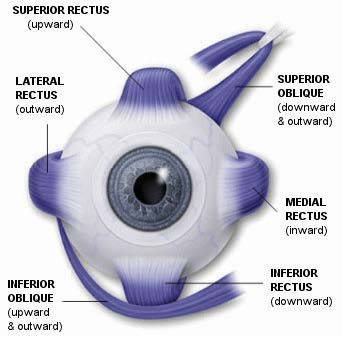
\includegraphics[width=0.4\textwidth]{../images/EOG_1.jpg}
\caption{Ocular muscles}
\label{eye}
\end{figure}

The human eye has 6 muscles attached to the exterior surface (Fig. \ref{eye}). These muscles are innervated by motor neurons that have electrical activities with a tonic component that controls eye position and a phasic component that controls the velocity of the movement. These muscles are grouped into three antagonistic pairs responsible for:
\begin{itemize}
	\item \textit{Horizontal movement}: medial rectus turns the eye toward the nose (adducts) and lateral rectus turns the eye away from the nose (abducts)
	\item \textit{Vertical movement}: superior rectus turns the eye up (elevates) with a slight inward rotation (intorts) and the inferior rectus turns the eye down (depresses) with a slight rotation away from the nose (extorts)
	\item \textit{Torsional movement}: superior oblique rotates the top of the eye towards the nose with a slight depression and the inferior oblique rotates the top of the eye away from the nose with a slight elevation
\end{itemize}

Electrically, the eye is a spherical "battery," with the positive terminal in the front (at the cornea), and the negative terminal behind the eyeball (at the retina). The potential between the front and back of the eyeball is about 0.4 to 1.0 mV. By placing electrodes on either side of the eye, you can measure eye movement (up to $\pm$70\degree, where 0\degree is in the front and $\pm$90\degree is directly lateral or vertical to the eyes). The electrodes measure the changes in potential as the cornea moves nearer or further from the recording electrodes. When the eye is looking straight ahead, it is about the same distance from either electrode, so the signal is essentially zero. When the cornea is closer to the positive electrode, that electrode records a positive different in voltage.\\

The integration of signals from different groups of neurons in the oculomotor system control five types of eye movement:
\subsection*{Saccades}
The fovea (focal point) is the region of the retina that sees in detail. Saccadic eye movements change the position of both eyes so that the image of interest falls on the fovea. When you read, your eyes and your brain have to work in synchrony. Your brain initiates and stops eye movement, and your eyes are sending information to your brain about what is in your visual field. If you need to see something different in your visual field, your brain has to signal your eye muscles to move them appropriately.\\

To compensate for poor vision that occurs during saccades, saccadic movements are quick with a velocity as high as 900\degree of movement/second. This rate can change depending on the signal the brain sends to your eyes. For example, if you read a word you do not understand, or are having trouble comprehending the material, your brain will need to tell your eyes to reread that material so it can make sense of it. On the other hand, if a passage is easy to read and comprehend, your eyes will sail over the words comparatively easily. This will affect the speed of reading, such that reading for simpler material is typically faster. These motions to reread and comprehend are called saccades, and will typically occur at a higher rate in more difficult reading materials.

\subsection*{Pursuit}
This eye movement keeps the fovea pointed at a moving target. There is an initial delay in pursuit movement because the signal from the eye has to be conducted through many synapses to the brain stem. Initially, when the object starts to move, a saccade helps the fovea catch up to the object until the pursuit movement begins to track the object.

\subsection*{Vergence}
This movement points the fovea of each eye onto an object when you look from a target that is distant to one that is closer, or vice versa. In vergence, the eyes rotate in opposite directions; eyes converge when looking from far to near, and diverge when looking from near to far. Vergence prevents double vision.

\subsection*{Vestibular Ocular Reflect (VOR)}
This reflex helps keep the image of the outside world stationary on the entire retina when the head moves. If you rotate your head to the left as you look at this page, your eyes rotate to the right. VOR is a phasic response that is faster than pursuit because it is a simple central reflex arc involving only 3 neurons. The signal that indicated the velocity of the head movement originates in the ear and goes through an efferent nerve and an interneuron on its way to the motor neurons of the oculomotor muscles. The muscles rotate the eyes at a velocity that matches the velocity of the head., thus keeping the image stationary on the retina.

\subsection*{Optokinetic Reflex}
This reflex is active when the full field of vision has moved across a large portion of the retina. Even though it is slower than VOR, it is better suited for slow and prolonged movements. This reflex can take place if a large object in your field of view is moving, giving you the sensation that you are moving in the opposite direction even though you are stationary. The device used to test this reflex is known as an optokinetic drum, which projects a series of rotating images on the wall of a small circular room.

\section*{Designing an Experiment}
This section describes the steps to correctly design and perform the laboratory activities for this week.
\begin{enumerate}
	\item \textit{State your specific question}: Select one question that you would like to address (you may use the list provided in the next section or create your own).
	\item \textit{Determine the general research question}: This should not be the specific question, but the general research question that you are trying to address in terms of physiological parameter. E.g. specific question: "how hard am I working when I run or walk?"  vs. general question: "does heart rate increase in response to exercise?"
	\item \textit{Formulate a hypothesis}: Make sure your hypothesis can be tested! You should be able to design an experiment (or set of experiments) that will provide evidence to support or refute your hypothesis.
	\item \textit{Determine your experiment design}: Before you start working on your experiments, familiarize yourselves with the way data is collected and how it is visualized. Look at the sample data (L10 files), and when you are comfortable with the data, record some values using your EOG setup to make sure you can replicate the values you just saw (some of these values will be used as controls, so spend some time collecting data).\\
		
		Consider all the factors that will play a role in your experiment (controlled variables, independent or experimental variables, and dependent or measured variables). Determine a time frame for your experiments, as well as an appropriate sample size. Clearly state what values you will measure. If needed, define a baseline setup or proof of concept that provides you with a positive or negative reference value and/or a baseline that allows you to determine what your recordings mean before you start recruiting subjects for your study. \textit{Modify your experimental design when needed.}
		
	\item \textit{Collect and analyze data}: For this experiment, compile a table with baseline (reference) values and collected values for the determined experimental conditions. Summarize this data with a graph or table, and if possible, perform a statistical analysis.
	\item \textit{Interpret data and make conclusions}: After analyzing the data, you must relate it back to your general research question. Make comments regarding the physiological meaning of your results and the broader implications of your findings.
\end{enumerate}

Before you begin your experiments, you will state a research question, propose a hypothesis, and design an experimental plan to follow. After that, data will be collected and analyzed in order to prove or disprove your hypothesis.\\

State a question that will allow you to demonstrate either saccades (reading difficulty) or pursuit (real vs. imaginary). Some example specific questions are as follows:\begin{itemize}
	\item Is your partner studying or reading a fun book?
	\item Is your partner paying attention to what they are reading?
	\item Your partner says they have an imaginary friend that keeps walking back and forth. Can they really see them or just imagine them?
	\item Is your partner following the bouncing ball or just pretending?
\end{itemize}

Indicate your \textbf{specific question}, \textbf{general research question}, and \textbf{hypothesis} on the handout. For your hypothesis, consider the following:\begin{itemize}
	\item How would you expect your variable to affect your results?
	\item Do you think there will be a difference between the two variables you are considering?
\end{itemize}

On the handout, clearly state your \textbf{experimental protocol} and \textbf{variables} to be measured. Please write additional parameters that you discussed for your experimental design at the bottom of the table; add more rows if necessary.

\section*{Experimental Methods}
In this exercise, the subject will perform tasks that will generate electrical activity in oculomotor muscles that are unique to different types of eye movement. We will examine the relationship between the type of eye movement and the different activities performed.\\

\subsection*{Electrode Setup}
\begin{enumerate}
	\item Attach one electrode in each of the following positions (Fig. \ref{setup1}):\begin{itemize}
		\item above your right eye
		\item below your right eye
		\item to the right of your right eye
		\item to the left of your left eye
		\item 2 electrodes on your forehead - above your left eye and nose (grounds)
	\end{itemize}
	
	\begin{figure}[h]
	\centering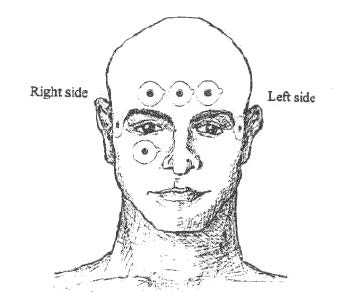
\includegraphics[width=0.4\textwidth]{../images/EOG_2.jpg}
	\caption{EOG electrode placement}
	\label{setup1}
	\end{figure}
	
	\item One lead set (SSL2) must be plugged into channel 1 and will measure the horizontal displacement. Connect the electrode on your right temple to the red cable, the one on the left temple to the white cable, and the one on your forehead to the ground black cable (Fig. \ref{setup2}). 
	
	\begin{figure}[h]
	\centering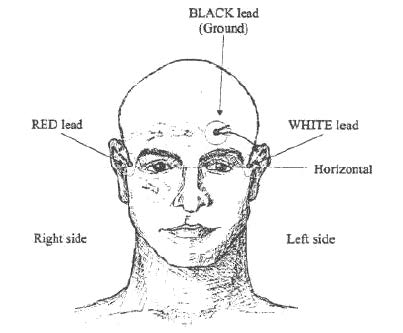
\includegraphics[width=0.4\textwidth]{../images/EOG_3.jpg}
	\caption{Lead placement for channel 1 (horizontal movement)}
	\label{setup2}
	\end{figure}
	
	\item The other lead set (SSL2) must be plugged into channel 2 and will measure the vertical displacement. Connect the electrode above your right eye to the red cable, the one below your right eye to the white cable, and the one on your forehead to the ground black cable (Fig. \ref{setup3}).
	
	\begin{figure}[h]
	\centering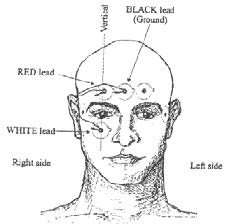
\includegraphics[width=0.4\textwidth]{../images/EOG_4.jpg}
	\caption{Lead placement for channel 2 (vertical movement)}
	\label{setup3}
	\end{figure}
	
	\item Position the subject 25-50 cm from the screen with their eyes aligned with the center of the screen.
	\item Open BIOPAC lesson L10 and click Calibrate. Following the calibration instructions on the screen and press Done to begin recording.
	\item Before you start recording data from your subjects, perform your baseline routine or proof of concept.
	
	\begin{info}
		If modifications to your testing protocol or experimental design are required, this is the step to make them. After this point, you begin data collection and all your subjects should be exposed to the same conditions.
	\end{info}
\end{enumerate}

\subsection*{Data Collection}
\begin{enumerate}
	\item If you need reference values, show a table with the baseline values measured. Otherwise, draw a sample of your data for each group and specify what values you will measure and why.
	\item Write down the instructions that you will provide to the subject before you begin the experiment. Make sure the instruction are concise and repeatable.
	\item Create a table will all experimental values measured. Make sure your table includes the subject number and the parameters you are planning to compare.
\end{enumerate}

\section*{Data Analysis}
\begin{enumerate}
	\item Choose a graph and/or table that summarizes your collected data.
	\item Perform a statistical analysis of your choosing.
	\item State whether or not your hypothesis is supported by the data. Be as specific as possible.
	\item Did your data have any interesting findings? If so, suggest a reason for these interesting findings.
	\item Were there factors not measured that you believe would affect the results? List these factors and justify why they would affect the results.
	\item What are the implications of your results? Relate your findings back to your understanding of physiology. Support your claims with literature if necessary.
\end{enumerate}
\end{document}
